% File: algo.tex
% Date: Sun Jun 23 01:54:26 2013 +0800
% Author: Yuxin Wu <ppwwyyxxc@gmail.com>
\section{算法说明}
\subsection{光线追踪及光照模型}
光线追踪的基本原理如下图所示.
\begin{figure}[H]
  \centering
  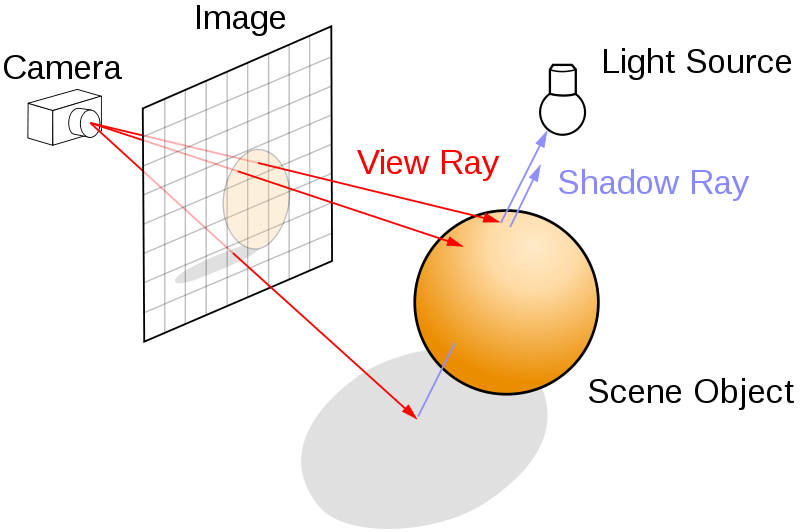
\includegraphics[scale=0.4]{res/ray_tracing.png}
\end{figure}

选定视点位置及一观察屏,从视点到屏上各点发出光线与空间中物体求交.
在交点处根据局部光照模型计算颜色,再递归的计算反射、透射光颜色,混合后显示在屏上.

此程序使用的局部光照模型为Phong模型,其主要公式为\cite{phong}:

\[  I_p = k_ai_a + \sum_{m\in lights} (k_d ( \overrightarrow{L_m} \cdot \overrightarrow{N} i_{m, d} + k_s(\overrightarrow{R_m}\cdot
  \overrightarrow{V})^{\alpha} i_{m, s}))  \]

其中$ k_s, k_d, k_a, \alpha$分别为物体表面该点处的高光系数,漫反射系数,环境光系数,亮度.
$ \overrightarrow{L_m}$为该点指向光源的向量, $ \overrightarrow{N}$为表面法向,
$ \overrightarrow{R_m}$为光源指向该点的光线经理想反射后的指向,
$ \overrightarrow{V}$为视点到表面交点处的向量.

\subsection{几何对象表示及计算}
程序支持了平面、球、三角面片、包围盒四类基本几何物体,
物体都需要各自拥有与光线求交的方法.

\begin{description}
  \item[光线]光线是一条射线,包含一个起始点及方向. 见\verb|include/geometry/ray.hh|
  \item[无穷平面]
    为了计算方便,使用平面法向及平面到原点的距离作为确定平面的方式.
    平面与光线求交时,首先通过光线指向判断是否相交,再通过
    光线在平面法向方向的投影长度计算交点.见\verb|include/geometry/infplane.hh, renderable/plane.cc|

  \item[球]球由球心及半径唯一确定.球与光线求交时,
    利用球心到它在光线所在直线上的投影的距离判断是否相交,在根据投影位置及勾股定理计算交点.
    求交时要考虑光线起始点在球内部的情形,以供计算相对折射率.见\verb|include/geometry/sphere.hh, renderable/sphere.cc|

  \item[三角面片]三角面片用三个顶点坐标存储.
    为了性能,与光线的求交参考了\cite{triangle, triangle_code}的算法及实现,其基本思想是求解满足
    方程
    \[  \overrightarrow{Orig} + t  \overrightarrow{Dir} = x \overrightarrow{v_1} + y  \overrightarrow{v_2} + (1 - x -
      y)\overrightarrow{v_3}, t > 0, x, y \in (0, 1), x + y \le 1\]
    的$ (t, x, y)$, 在求交时同时能得到交点的重心坐标\footnote{\url{https://en.wikipedia.org/wiki/Barycentric\_coordinate\_system}}
    ,便于之后进行法向插值.见\verb|include/renderable/face.hh, renderable/face.cc|

  \item[轴平行包围盒]
    轴平行包围盒用最小坐标与最大坐标两个向量存储.
    为了效率,包围盒与光线求交部分参考了\cite{aabb}的算法.
    其基本思想是对每个面逐一计算并更新交点.见\verb|geometry/aabb.hh|
\end{description}


\subsection{视图模型}
一个视图应包括视点及屏幕,且应使视点在屏幕的中轴线上.
视图类\verb|View|存储了视点坐标,屏幕中心坐标,屏幕尺寸,屏幕边沿的空间指向,
并保证视点到屏幕中心的连线与屏幕边沿指向垂直.
这样可以方便的进行视图旋转,视图平移,缩放等导航操作.见\verb|include/view.hh, view.cc|

\subsection{KD树}
KD树是一种空间划分树,原本用于在K维空间中快速查找点,可利用在光线追踪中对物体及其包围盒进行索引.
基本方法是,树中每个节点对应一个包围盒,选取一个轴平行平面将包围盒一分为二作为两个子节点,叶节点存储包围盒中的物体.
注意与切分面相交的物体在两子节点中都应维护.

\subsubsection{建树}
传统的KD树中,按照使两边点的个数尽量接近的原则选取切分平面,这是由于假设了各个点被查询的概率均等.
在光线追踪中,一般采用面积启发式的平面选取方式\cite{kdtree},选取切平面使得
两个子节点的包围盒表面积与包含物体个数的积之和尽量大,这样可以使KD树在查询时效率更高.
但启发式的建树需要枚举切分平面,计算包含物体个数,复杂度较高.
直接的枚举为$ O(n^2)$复杂度,本程序实现了\cite{kdtree}中提供的$ O(n \log^2 n)$算法.
对于20W面片的龙模型\footnote{models/fixed.perfect.dragon.100K.0.07.obj},
采用不同方法单线程建树的用时及在几个固定视角渲染耗时如下(单位: 秒):

\begin{table}[H]
  \begin{threeparttable}

    \begin{tabular}{c|c|c|c|c|c|c}
      \shline
      & 建树 & 视角1 & 视角2 & 视角3 & 视角4 & 视角5 \\ \hline
      二分建树(终止:100层,15个)  & 0.6  & 1.93  & 2.51  & 3.26  & 4.38  & 5.89  \\ \hline
      SAH建树(终止:100层,20个) & 5.41 & 0.29  & 0.37  & 0.45  & 0.59  & 0.78    \\ \hline
      SAH建树(终止:100层,15个) & 7.82 & 0.24  & 0.33  & 0.41  & 0.52  & 0.68    \\ \shline
    \end{tabular}
    \begin{tablenotes}
      \footnotesize
    \item 注: 1.建树时,以树深度及当前节点所管理的物体个数作为建树结束的判定条件.
    \item 2.此实验的视角1为\verb|main.cc|中\verb|test_kdtree()|提供的视角,其余视角由视角1 zoom in依次得到.
    \item 3.可在\verb|lib/kdtree.cc|中通过注释\verb|KDTree::build()|函数中相应代码切换两种建树算法.
    \end{tablenotes}
  \end{threeparttable}
\end{table}

由表可见SAH建树的查询效率有很大提高,但建树缓慢. 建树效率与渲染效率之间存在trade-off,可以通过改变终止条件来调整.

另外,不使用KD树时,视角1渲染时间约为800s.(不使用KD树时各像素所需时间大致相同,可由部分渲染时间估算总时间).

\subsubsection{求交}
求交的基本方法为,递归寻找两子树中最近\underline{物体}的交点,取较近者为结果返回.

实现时,在每个节点处保存了当前节点的两个孩子的切分平面,这样可以预先判断出离
光线较近的包围盒,若与其内物体相交则不用考虑另一包围盒.
使用此方法应注意,若光线与较近包围盒所管理的物体相交,应确认与最近物体的交点是否被较近包围盒\underline{包含}.
因为若不包含,则光线首先打到的物体可能并不是此物体,而是第二个包围盒管理的物体.

\subsection{纹理}
一种纹理相当于一个二维坐标到表面属性的映射.
表面属性除Phong模型参数外,还包括了透明度,用于折射判定,以及发光强度,用于全局光照模型.
程序实现了均匀纹理、网格纹理、图片纹理三类纹理,并可通过继承\verb|Texture|类进行扩展.

对于一个物体,由其自己管理三维坐标到二维坐标的映射.
对于平面,采用平面上的二维欧式坐标. 球体采用其极坐标.
网格未支持二维纹理,仅可以使用均匀纹理.

\subsection{法向插值}
\label{sec:smooth}
法向插值可以使三角网格表面更光滑,只需找到一个面片上的连续函数,就可以得到较好的效果.
此程序采用了线性插值.

在读入网格数据后,令各顶点法向为其相邻各面法向的平均.
在面片与光线求交后,根据交点的重心坐标及面片顶点的法向,即可插值出交点法向.
效果见\figref{smooth}, \figref{simplify}.

\subsection{抗锯齿}
\begin{enumerate}
  \item 使用Beer-Lambert定律\cite{beer},使得光线亮度按传播距离指数衰减,可以有效消除远处纹理密集处的畸形.
    见\figref{first}与\figref{beer}的对比.

  \item 使用全屏抗锯齿(FSAA),对图片整体应用卷积盒$\begin{bmatrix}1 & 2 & 1\\2 & 4 & 2\\1 & 2 & 1\end{bmatrix} $,
    消除直线锯齿的同时使图片模糊,影响视觉效果.

  \item 对每一像素,计算其与周围像素距离平方之和,若小于某一阈值则应用如上卷积盒,略有效果. 见\verb|CVRender::antialias()|
\end{enumerate}

\subsection{软阴影}
\label{sec:soft}
对场景中每一点光源,将其替换为点周围的多个密集点光源以模拟面光源的效果,
即可实现软阴影.效果如\figref{soft}所示. 实现见\verb|Space::add_light()|.

\subsection{景深}
程序中景深\footnote{\url{http://en.wikipedia.org/wiki/Depth\_of\_field}}
的实现方法为,以焦平面作为屏幕,取焦平面与视点之间某处建一感光器平面.
对视点到焦平面的每条光线,在其与感光器的交点周围随机采多个样本点,以这些样本点为观察点向
屏幕同一位置发射光线并执行光线追踪,以各样本点颜色的平均值作为最终颜色.
这样就可以使得焦平面上物体清晰,而其余位置模糊.


\verb|main.cc|中的\verb|dof_ball_scene()|生成一个演示景深的场景,场景中
可通过键盘控制焦平面位置,详见\tabref{navigate}.demo目录中有景深的演示视频.

随机取点会造成焦平面以外有无规律噪点,在生成视频后会比较明显,
因而对输出图像统一做了高斯模糊,使噪点不太明显.

\subsection{小量处理}
在如下情形需要特别注意实数运算中的误差.
\begin{enumerate}
  \item 反射折射交点

    考虑光线斜射平面的情形,若交点由于误差落在了平面异侧,则反射光仍会打到平面,
    若落在了平面同侧,则透射光仍会打到平面.因而计算反射光线时,
    应将其起始点回退EPS,计算透射光线时,应将其起始点前进EPS.

  \item 平行判定

    判定直线与面片或平面是否平行时,利用直线与法线点乘的绝对值$<$EPS判定,
    否则可能导致交点坐标过大.

  \item KD树

    建树时,对于包围盒相交的判定应略微宽松,与包围盒距离$<$EPS的物体都应归入包围盒管理,
    查询时对光线与面片求交也可判的宽松一些,否则渲染的图片中容易出现黑点.

    对面片求包围盒时应注意最小值应减去EPS,最大值应加上EPS,
    否则可能出现0体积包围盒,影响算法实现.
\end{enumerate}

\subsection{网格简化}
网格的坍缩简化算法参考\cite{mesh}实现.
基本思路是,对每对顶点估算出简化代价,每次选取代价最小的顶点对执行简化操作,操作后更新相关的代价值.

由于算法具有优先队列结构,因此使用了\verb|std::priority_queue|进行堆加速.
但由于需要执行堆元素修改操作,因而对堆结构进行了如下处理:

对每个顶点,维护它相邻顶点中最适合坍缩的顶点指针.
堆元素存储一顶点指针及它与相应邻点的坍缩代价,另有一时间戳.
堆元素按照坍缩代价保持堆性质,坍缩一对顶点后更新了附近顶点的最优代价,就将新的值打上新的时间戳压入堆中,
而取堆顶元素时,若从时间戳发现其不是最新就抛弃.这样就可以替代修改操作.见\verb|include/mesh_simplifier.hh, mesh_simplifier.cc|

对于20万面片的龙模型\footnote{models/fixed.perfect.dragon.100K.0.07.obj},
简化掉80\%的面片需要2.37s, 而不用堆加速时需要55s.效果见\figref{simplify}.

\subsection{多线程}
\begin{enumerate}
  \item 对生成图片中每个像素,显然其计算相互独立,使用openmp及C++11的\verb|std::thread|两种方式对其进行多线程优化,
    效果差不多.见\verb|CVViewer::render_all()|.

  \item 建树时,两子树的创建可以并行执行.
    测试表明对根节点的两子节点并行建树有效,而对深层节点并行建树得不偿失.
    另外,$O(\log^2 n)$的建树中有一步需对各物体每一维度上的坐标排序,这是效率的瓶颈所在.
    不同维度的排序可以并行执行,经测试也只对根节点比较有效.
    这两处并行都使用C++11的\verb|std::future|实现,效率提升了约30\%.

  \item 网格简化中,对各节点代价的更新可以并行完成,效率略有提高.
\end{enumerate}
